\documentclass[paperwidth=30in,paperheight=40in,portrait,fontscale=0.3]{baposter}

% Encoding.
\usepackage[utf8]{inputenc}
\usepackage{graphicx, wrapfig} % Required for including images
\usepackage{float}
\usepackage{hyperref}
\usepackage{helvet}
\renewcommand{\familydefault}{\sfdefault}
\usepackage[font=small,labelfont=bf,justification=centering]{caption} % Required for specifying captions to tables and figures
\usepackage{subcaption} % put figures side by side
\usepackage{lipsum}
\usepackage{enumerate}

\newcommand{\compresslist}{ % Define a command to reduce spacing within itemize/enumerate environments, this is used right after \begin{itemize} or \begin{enumerate}
\setlength{\itemsep}{1pt}
\setlength{\parskip}{0pt}
\setlength{\parsep}{0pt}
}

% Defines the color used for content box headers
\definecolor{lightblue}{cmyk}{0.83,0.24,0,0.16}
\definecolor{ghostwhite}{rgb}{0.97, 0.97, 1.0}
\definecolor{lightseagreen}{rgb}{0.13, 0.7, 0.67}

%%%%%%%%%%%%%%%%%%%%%%%%%%%%%%%%%%%%%%%%%%%%%%%%%%%%%%%%%%%%%%%%%%%%%%%%%%%%%%
%%% Begin of Document
%%%%%%%%%%%%%%%%%%%%%%%%%%%%%%%%%%%%%%%%%%%%%%%%%%%%%%%%%%%%%%%%%%%%%%%%%%%%%%
\frenchspacing

\begin{document}

\hyphenation{resolution occlusions}
%%
\begin{poster}%
  % Poster Options
  {
  % Show grid to help with alignment
  grid=false,
  % Column spacing
  colspacing=1em,
  % Color style
  bgColorOne=ghostwhite,
  bgColorTwo=white,
  borderColor=lightblue,
  headerColorOne=lightblue,
  headerColorTwo=lightblue,
  headerFontColor=white,
  boxColorOne=white,
  boxColorTwo=lightblue,
  % Format of textbox
  textborder=rounded,
%  textborder=faded,
  % Format of text header
  eyecatcher=true,
  headerborder=closed,
  columns=2,
  headerheight=4cm,
%  textfont=\sc, An example of changing the text font
  headershape=rounded,
  headershade=shadelr,
  headerfont=\Large\bf, %Sans Serif
  textfont={\setlength{\parindent}{1.5em}\large},
  boxshade=plain,
%  background=shade-tb,
  background=plain,
  linewidth=1pt
  }
  { % Left Eye Catcher - GT logo
	
\includegraphics[width=3.5cm]{img/gt-logo-gold.png}
  }
  % Title
  	{\bf{Learning about the Attention Mechanism and the Transformer model}}
  % Authors
  {\textbf{\null\hfill Baptiste Amato  \hfill Alexis Durocher \hfill Gabriel Hurtado \hfill\null}\\
  	\vspace{-0.3em }
	\textbf{\null\hfill Alexandre Jouandin \hfill Vincent Marois \hfill\null}\\

  %\texttt{\large\{baptiste.amato, adurocher3, gabriel.hurtado, alexandre.jouandin, vincent.marois\}@gatech.edu}\\

	{\large\underline{Spring 19 -- CS 7643 Deep Learning -- Prof. Zsolt Kira}}\\
  }

  %{ % Right Eye Catcher
	%\includegraphics[width=3.5cm]{}
  %}

%%%%%%%%%%%%%%%%%%%%%%%%%%%%%%%%%%%%%%%%%%%%%%%%%%%%%%%%%%%%%%%%%%%%%%%%%%%%%%%

\headerbox{Motivation}{name=motivations,column=0,row=0}{

	\begin{itemize}
	  \compresslist
	  \item Transformer~\cite{vaswani2017attention} model is a SoTA Machine Translation model,
	  \item No recurrence, only uses the Attention Mechanism~\cite{bahdanau2014neural},
	  \item Known to be difficult to implement correctly,
	  \item[$\Rightarrow$] What can we learn about the model?
	\end{itemize}

}

\headerbox{The Dataset}{name=dataset, column=0, below=motivations}{

	\begin{itemize}
	  \compresslist
	  \item IWSLT 2016 TED talk translation task (French $\rightarrow$ English),
	  \item 220k train samples, 1025 validation, XXX test,
	  \item Average sentence length: 20 (train) -- 21 (val).
	\end{itemize}

	\vspace{-20pt}
	\begin{figure}[H]
	\begin{subfigure}{0.5\textwidth}
		\centering
		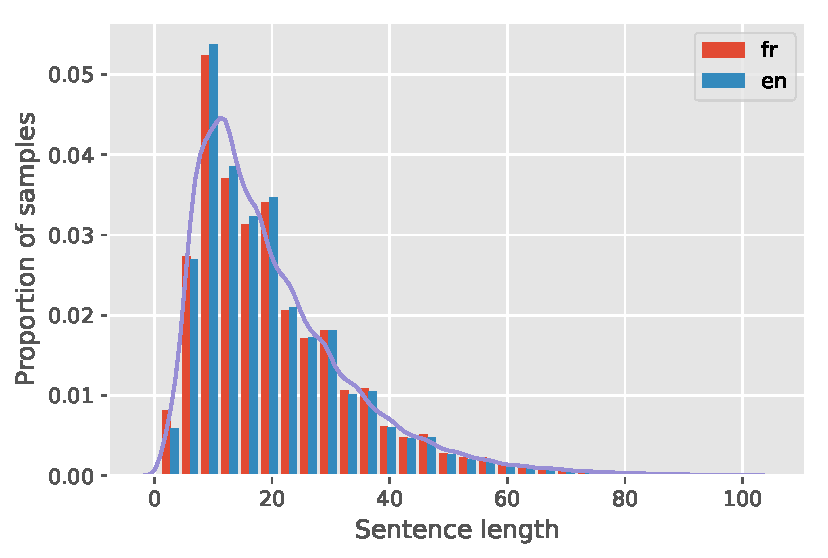
\includegraphics[width=0.9\linewidth]{img/seq_length_distribution.pdf}
		\caption{Sentence Length Distribution.}
		\label{fig:seq-length-distrib}
	\end{subfigure}%
	\begin{subfigure}{0.5\textwidth}
		\centering
		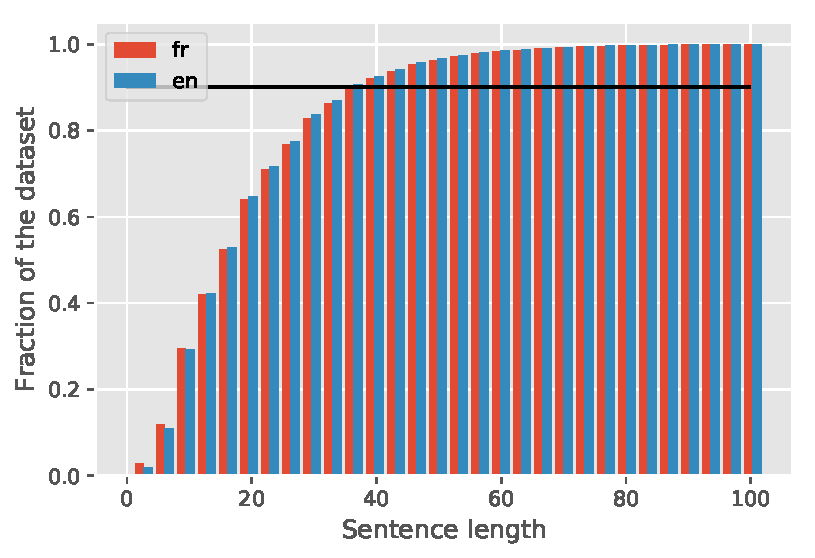
\includegraphics[width=0.9\linewidth]{img/seq_length_distribution_cum.pdf}
		\caption{Cumulated Distribution.}
		\label{fig:cum-seq-length-distrib}
	\end{subfigure}
	\end{figure}

}

\headerbox{The Transformer Model}{name=model, column=0, below=dataset}{

  \begin{figure}[H]
    \centering
    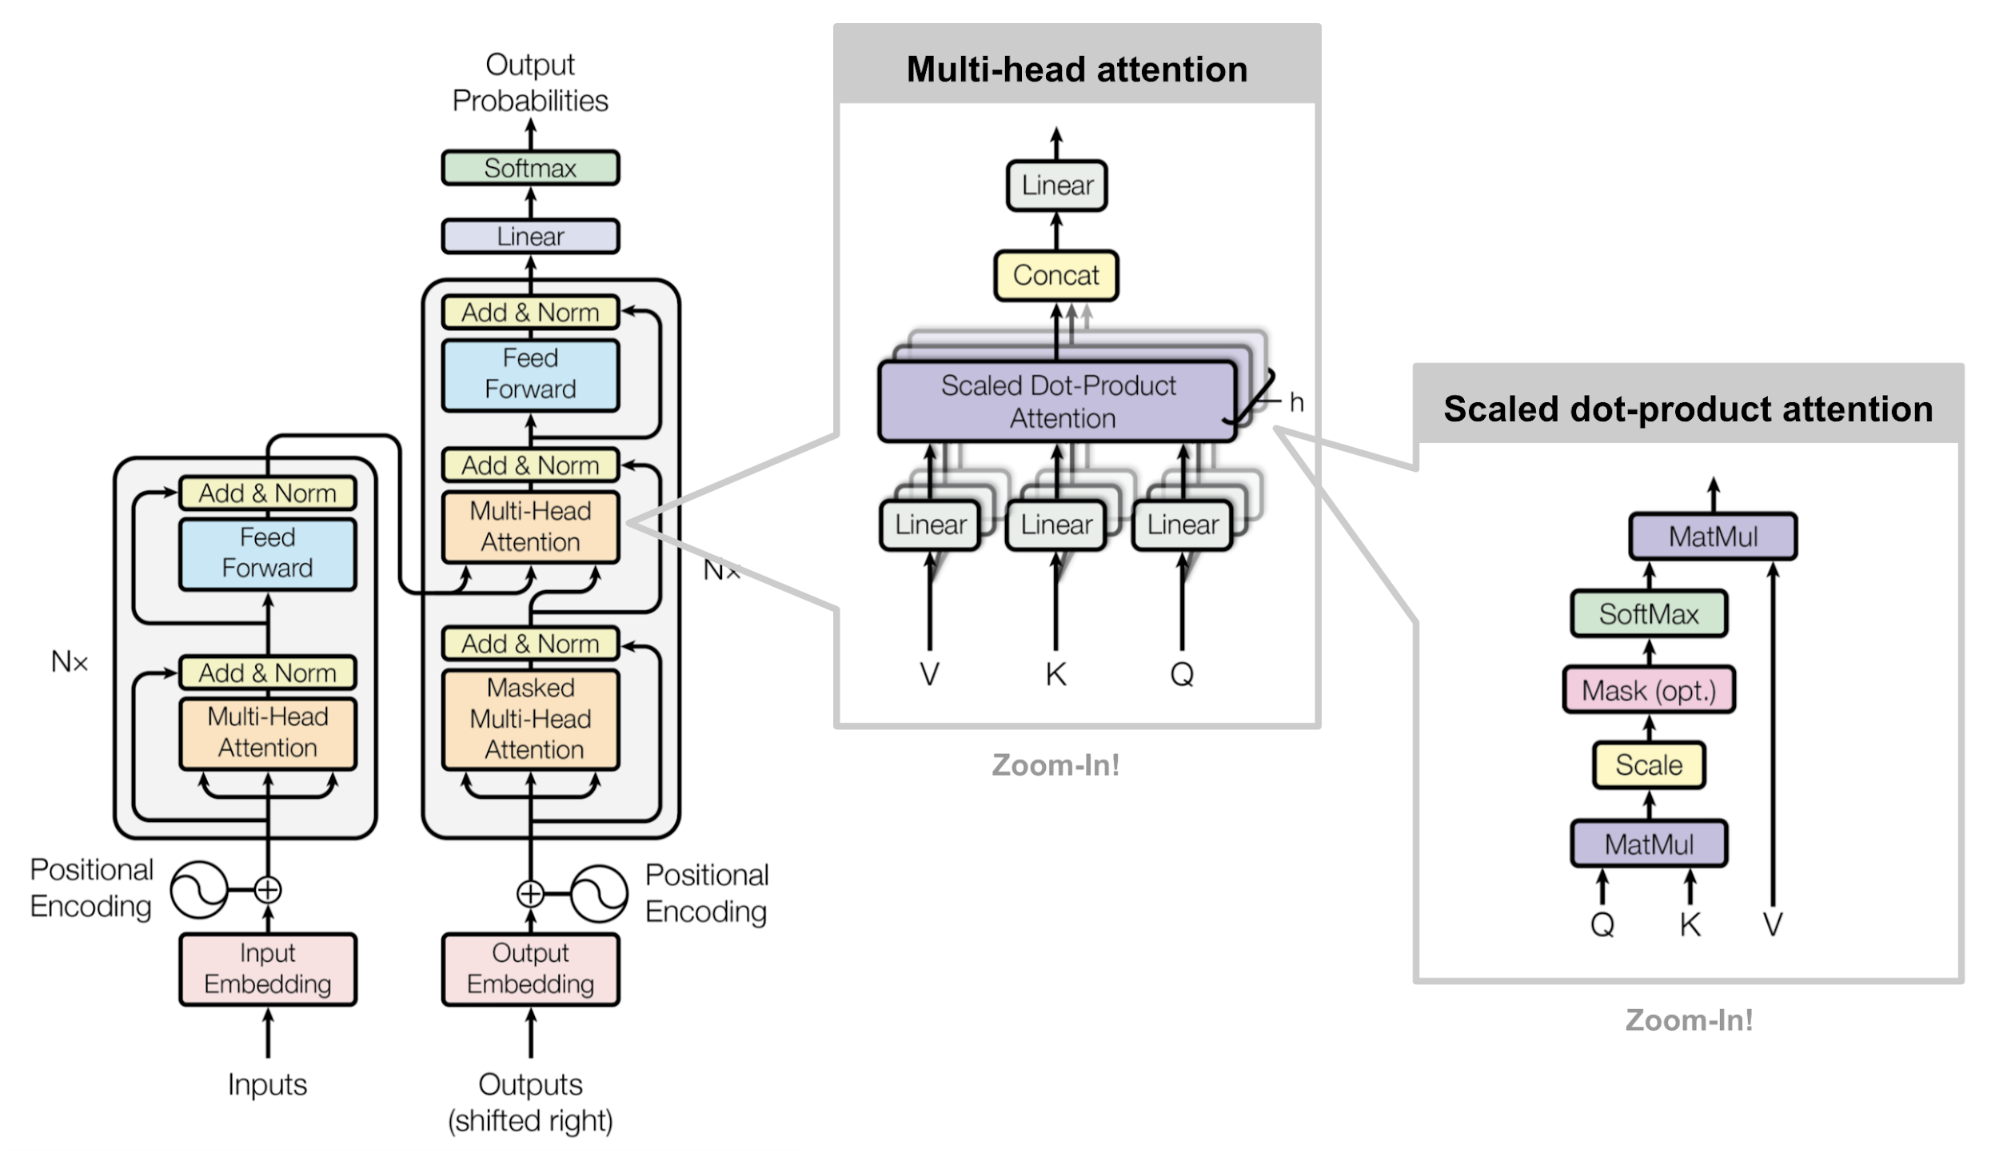
\includegraphics[width=\textwidth]{img/transformer.png}
    \caption{The Transformer model Architecture and the Attention Heads.}
    \label{fig:model}
  \end{figure}
  \vspace{-20pt}
  \begin{itemize}
    \compresslist
    \item Encoder-Decoder architecture,
    \item Less computation-heavy than RNNs for translation.
  \end{itemize}

}

\headerbox{References}{name=links, column=0, below=model}{
  \small
  \vspace{-8pt}
  \renewcommand{\refname}{}
  \bibliographystyle{alpha}
  \bibliography{references.bib}

}

\headerbox{Experiments}{name=experiments, column=1}{
	\begin{itemize}
		\compresslist
		\item Model working on the copy task (\texttt{inputs = outputs})
	\end{itemize}
  \vspace{-20pt}
	\begin{figure}[H]
		\centering
		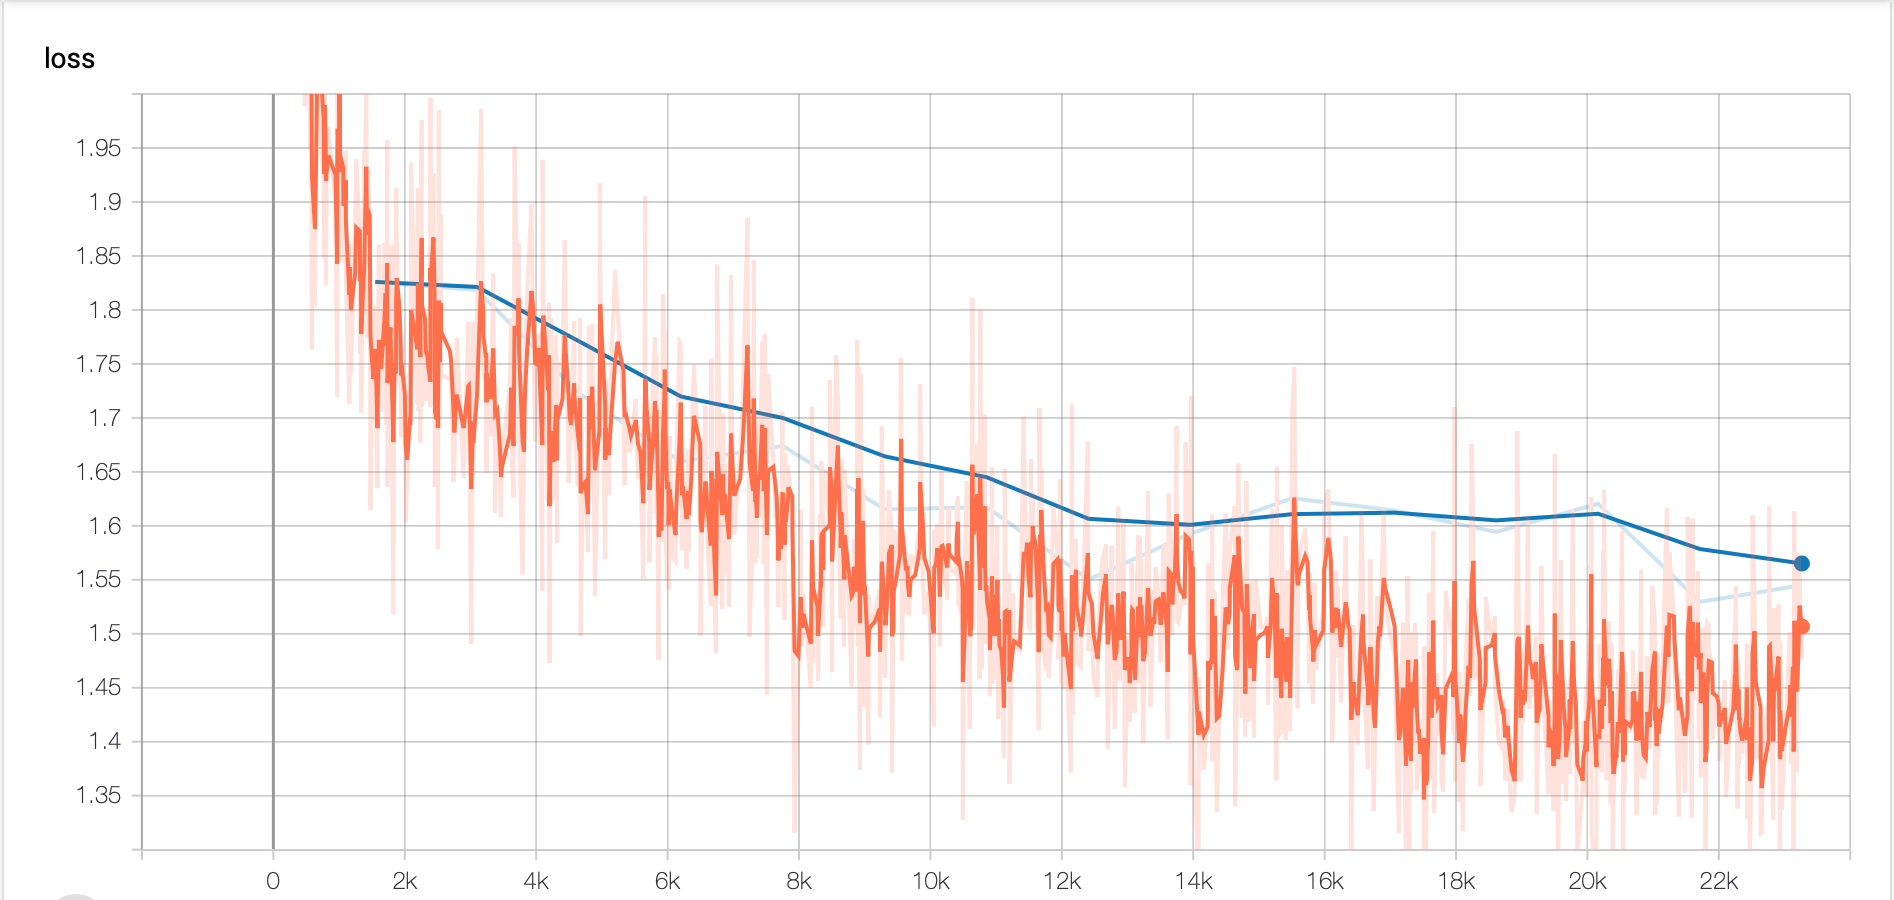
\includegraphics[width=\textwidth]{img/training.png}
		\caption{Training and Validation loss on 40\% of the IWSLT dataset.}
		\label{fig:training}
	\end{figure}

}

\headerbox{Memory Use Analysis}{name=memory-use, column=1, below=experiments}{
\vspace{-10pt}
\begin{figure}[H]
  \centering
  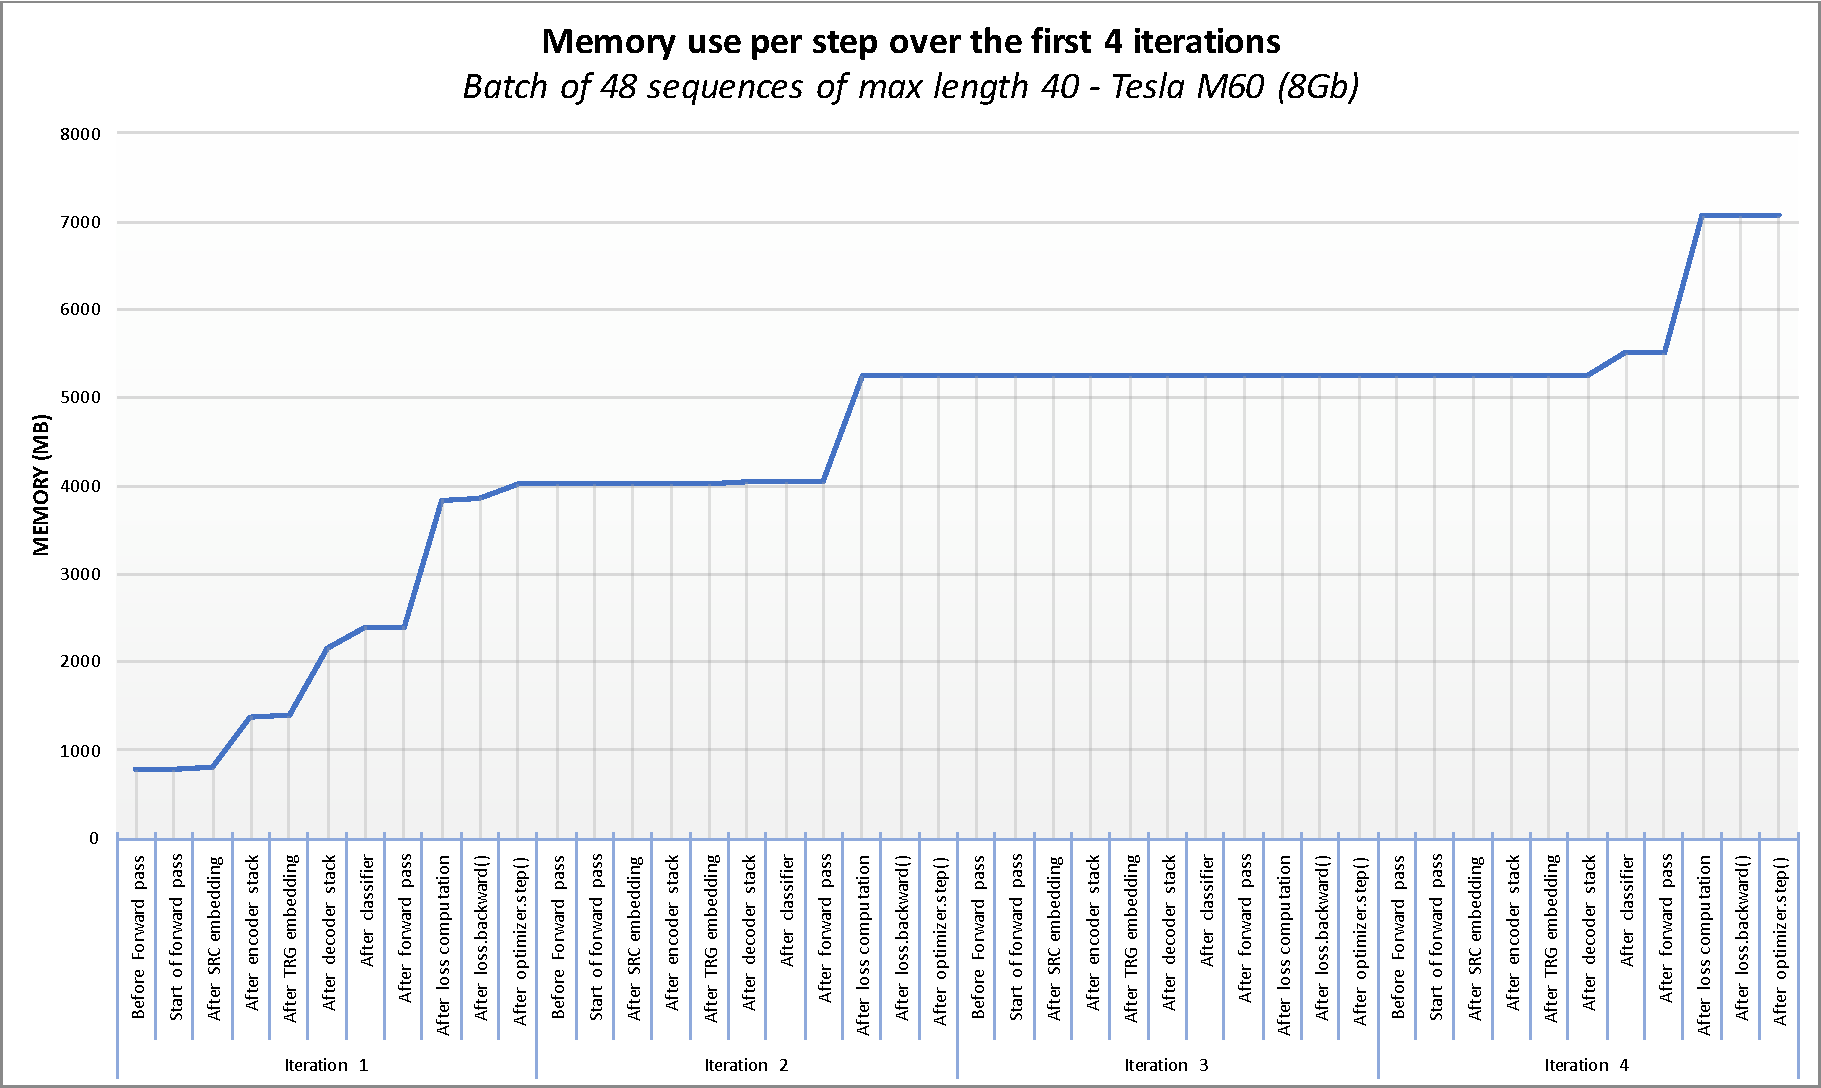
\includegraphics[width=\linewidth]{img/precise-memory-use-4-iterations.pdf}
  \caption{GPU Memory Use over the $1^{st}$ 4 iterations.}
  \label{fig:mem-use-4-iters}
\end{figure}
\vspace{-20pt}
\begin{itemize}
  \compresslist
  \item Initial increase of memory use, particularly when computing loss
  \item Stabilization over epoch at $\sim$6 Gb
  \item[$\Rightarrow$] PyTorch most likely optimizing in the background
\end{itemize}

% \begin{figure}
%   \centering
%   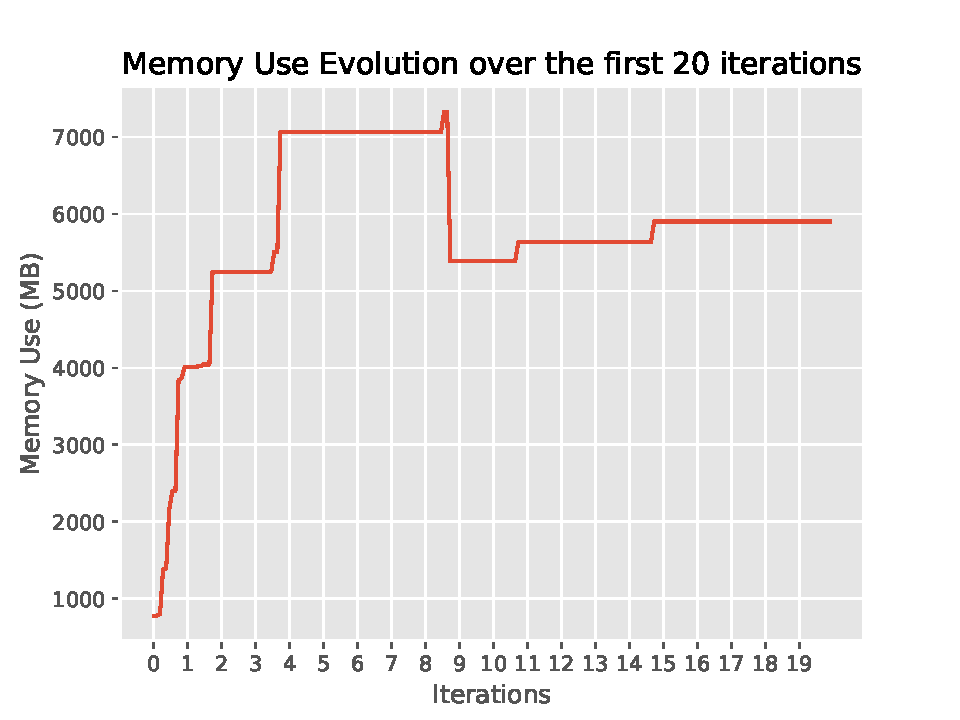
\includegraphics[width=\linewidth]{img/memory-use-20-iterations.pdf}
%   \caption{GPU Memoru use over the $1^{st}$ 20 iterations.}
%   \label{fig:mem-use-20-iters}
% \end{figure}


}

\headerbox{Conclusion}{name=results, column=1, below=memory-use}{
\lipsum[2]
}



\end{poster}

\end{document}
